\documentclass[]{article}
\usepackage{lmodern}
\usepackage{amssymb,amsmath}
\usepackage{ifxetex,ifluatex}
\usepackage{fixltx2e} % provides \textsubscript
\ifnum 0\ifxetex 1\fi\ifluatex 1\fi=0 % if pdftex
  \usepackage[T1]{fontenc}
  \usepackage[utf8]{inputenc}
\else % if luatex or xelatex
  \ifxetex
    \usepackage{mathspec}
  \else
    \usepackage{fontspec}
  \fi
  \defaultfontfeatures{Ligatures=TeX,Scale=MatchLowercase}
  \newcommand{\euro}{€}
\fi
% use upquote if available, for straight quotes in verbatim environments
\IfFileExists{upquote.sty}{\usepackage{upquote}}{}
% use microtype if available
\IfFileExists{microtype.sty}{%
\usepackage{microtype}
\UseMicrotypeSet[protrusion]{basicmath} % disable protrusion for tt fonts
}{}
\usepackage[margin=1in]{geometry}
\usepackage{hyperref}
\PassOptionsToPackage{usenames,dvipsnames}{color} % color is loaded by hyperref
\hypersetup{unicode=true,
            pdftitle={Homework 2},
            pdfauthor={Group 1},
            pdfborder={0 0 0},
            breaklinks=true}
\urlstyle{same}  % don't use monospace font for urls
\usepackage{color}
\usepackage{fancyvrb}
\newcommand{\VerbBar}{|}
\newcommand{\VERB}{\Verb[commandchars=\\\{\}]}
\DefineVerbatimEnvironment{Highlighting}{Verbatim}{commandchars=\\\{\}}
% Add ',fontsize=\small' for more characters per line
\usepackage{framed}
\definecolor{shadecolor}{RGB}{248,248,248}
\newenvironment{Shaded}{\begin{snugshade}}{\end{snugshade}}
\newcommand{\KeywordTok}[1]{\textcolor[rgb]{0.13,0.29,0.53}{\textbf{{#1}}}}
\newcommand{\DataTypeTok}[1]{\textcolor[rgb]{0.13,0.29,0.53}{{#1}}}
\newcommand{\DecValTok}[1]{\textcolor[rgb]{0.00,0.00,0.81}{{#1}}}
\newcommand{\BaseNTok}[1]{\textcolor[rgb]{0.00,0.00,0.81}{{#1}}}
\newcommand{\FloatTok}[1]{\textcolor[rgb]{0.00,0.00,0.81}{{#1}}}
\newcommand{\ConstantTok}[1]{\textcolor[rgb]{0.00,0.00,0.00}{{#1}}}
\newcommand{\CharTok}[1]{\textcolor[rgb]{0.31,0.60,0.02}{{#1}}}
\newcommand{\SpecialCharTok}[1]{\textcolor[rgb]{0.00,0.00,0.00}{{#1}}}
\newcommand{\StringTok}[1]{\textcolor[rgb]{0.31,0.60,0.02}{{#1}}}
\newcommand{\VerbatimStringTok}[1]{\textcolor[rgb]{0.31,0.60,0.02}{{#1}}}
\newcommand{\SpecialStringTok}[1]{\textcolor[rgb]{0.31,0.60,0.02}{{#1}}}
\newcommand{\ImportTok}[1]{{#1}}
\newcommand{\CommentTok}[1]{\textcolor[rgb]{0.56,0.35,0.01}{\textit{{#1}}}}
\newcommand{\DocumentationTok}[1]{\textcolor[rgb]{0.56,0.35,0.01}{\textbf{\textit{{#1}}}}}
\newcommand{\AnnotationTok}[1]{\textcolor[rgb]{0.56,0.35,0.01}{\textbf{\textit{{#1}}}}}
\newcommand{\CommentVarTok}[1]{\textcolor[rgb]{0.56,0.35,0.01}{\textbf{\textit{{#1}}}}}
\newcommand{\OtherTok}[1]{\textcolor[rgb]{0.56,0.35,0.01}{{#1}}}
\newcommand{\FunctionTok}[1]{\textcolor[rgb]{0.00,0.00,0.00}{{#1}}}
\newcommand{\VariableTok}[1]{\textcolor[rgb]{0.00,0.00,0.00}{{#1}}}
\newcommand{\ControlFlowTok}[1]{\textcolor[rgb]{0.13,0.29,0.53}{\textbf{{#1}}}}
\newcommand{\OperatorTok}[1]{\textcolor[rgb]{0.81,0.36,0.00}{\textbf{{#1}}}}
\newcommand{\BuiltInTok}[1]{{#1}}
\newcommand{\ExtensionTok}[1]{{#1}}
\newcommand{\PreprocessorTok}[1]{\textcolor[rgb]{0.56,0.35,0.01}{\textit{{#1}}}}
\newcommand{\AttributeTok}[1]{\textcolor[rgb]{0.77,0.63,0.00}{{#1}}}
\newcommand{\RegionMarkerTok}[1]{{#1}}
\newcommand{\InformationTok}[1]{\textcolor[rgb]{0.56,0.35,0.01}{\textbf{\textit{{#1}}}}}
\newcommand{\WarningTok}[1]{\textcolor[rgb]{0.56,0.35,0.01}{\textbf{\textit{{#1}}}}}
\newcommand{\AlertTok}[1]{\textcolor[rgb]{0.94,0.16,0.16}{{#1}}}
\newcommand{\ErrorTok}[1]{\textcolor[rgb]{0.64,0.00,0.00}{\textbf{{#1}}}}
\newcommand{\NormalTok}[1]{{#1}}
\usepackage{longtable,booktabs}
\usepackage{graphicx,grffile}
\makeatletter
\def\maxwidth{\ifdim\Gin@nat@width>\linewidth\linewidth\else\Gin@nat@width\fi}
\def\maxheight{\ifdim\Gin@nat@height>\textheight\textheight\else\Gin@nat@height\fi}
\makeatother
% Scale images if necessary, so that they will not overflow the page
% margins by default, and it is still possible to overwrite the defaults
% using explicit options in \includegraphics[width, height, ...]{}
\setkeys{Gin}{width=\maxwidth,height=\maxheight,keepaspectratio}
\setlength{\parindent}{0pt}
\setlength{\parskip}{6pt plus 2pt minus 1pt}
\setlength{\emergencystretch}{3em}  % prevent overfull lines
\providecommand{\tightlist}{%
  \setlength{\itemsep}{0pt}\setlength{\parskip}{0pt}}
\setcounter{secnumdepth}{5}

%%% Use protect on footnotes to avoid problems with footnotes in titles
\let\rmarkdownfootnote\footnote%
\def\footnote{\protect\rmarkdownfootnote}

%%% Change title format to be more compact
\usepackage{titling}

% Create subtitle command for use in maketitle
\newcommand{\subtitle}[1]{
  \posttitle{
    \begin{center}\large#1\end{center}
    }
}

\setlength{\droptitle}{-2em}
  \title{Homework 2}
  \pretitle{\vspace{\droptitle}\centering\huge}
  \posttitle{\par}
  \author{Group 1}
  \preauthor{\centering\large\emph}
  \postauthor{\par}
  \date{}
  \predate{}\postdate{}


\usepackage{relsize}
\usepackage{setspace}
\usepackage{amsmath,amsfonts,amsthm}
\usepackage[sfdefault]{roboto}
\usepackage[T1]{fontenc}
\usepackage{float}

% Redefines (sub)paragraphs to behave more like sections
\ifx\paragraph\undefined\else
\let\oldparagraph\paragraph
\renewcommand{\paragraph}[1]{\oldparagraph{#1}\mbox{}}
\fi
\ifx\subparagraph\undefined\else
\let\oldsubparagraph\subparagraph
\renewcommand{\subparagraph}[1]{\oldsubparagraph{#1}\mbox{}}
\fi

\begin{document}
\maketitle

{
\setcounter{tocdepth}{2}
\tableofcontents
}
\begin{center}
\topskip0pt
\vspace*{\fill}
\bigskip
\bigskip
\bigskip
Prepared for:\\
\medskip
Dr. Nathan Bastian\\
\smallskip
City University of New York, School of Professional Studies - Data 621\\
\bigskip
Prepared by:\\
\medskip
Group 1\\ 
\medskip
Senthil Dhanapal\\ 
\smallskip
Yadu Chittampalli\\
\smallskip
Christophe Hunt\\  
\vspace*{\fill}
\end{center}

\newpage

\section{Data Source}\label{data-source}

The data is a set of actual classes and predicted classes as provided by
Dr.~Nathan Bastian for this exercise. We uploaded the data to our public
GitHub repository for ease of access.

\section{Data Explained and Confusion
Matrix}\label{data-explained-and-confusion-matrix}

We will be using the following columns from the data source:

\begin{itemize}
\tightlist
\item
  class: the actual class for the observation
\item
  scored.class: the predicted class for the observation (based on a
  threshold of 0.5)
\item
  scored.probability: the predicted probability of success for the
  observation
\end{itemize}

The raw confusion matrix for our scored data set is represented the
following table. The rows represent the actual classes and the columns
represent the predicted classes.

\begin{longtable}[c]{@{}lcc@{}}
\toprule
& Predicted Failure & Predicted Success\tabularnewline
\midrule
\endhead
Actual Failure & 119 & 5\tabularnewline
Actual Success & 30 & 27\tabularnewline
\bottomrule
\end{longtable}

A visual representation of the confusion matrix is presented in the
below figure.

\begin{center}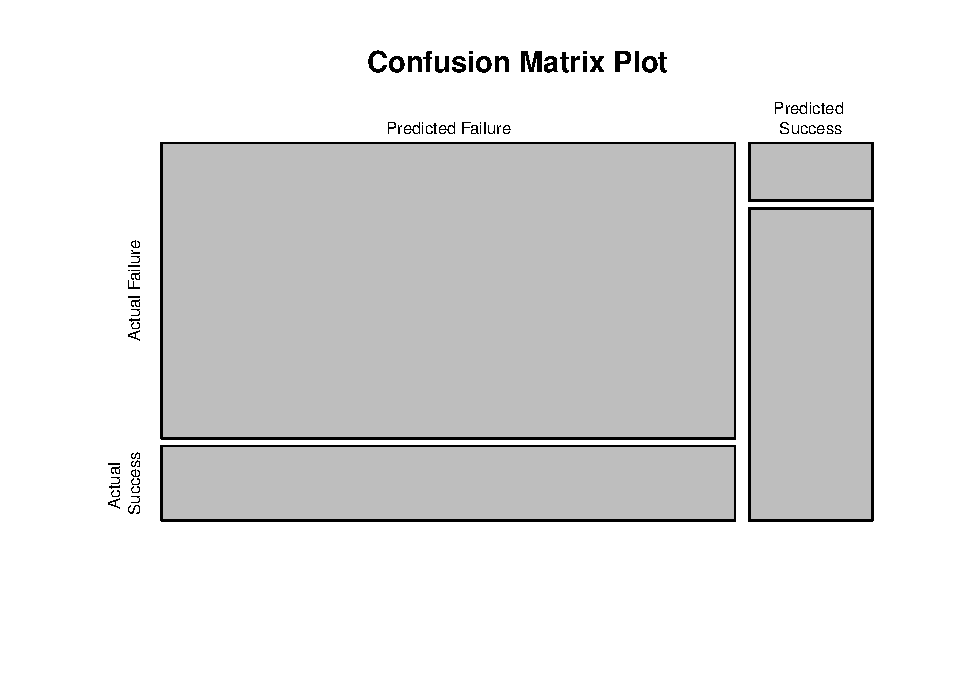
\includegraphics{Homework_2_files/figure-latex/unnamed-chunk-3-1} \end{center}

\section{Function for Accuracy of
Predictions}\label{function-for-accuracy-of-predictions}

We developed a function that takes the data set as a dataframe, with
actual and predicted classifications identified, and returns the
accuracy of the predictions.

Accuracy is determined by the below formula:

\[
\begin{aligned}
Accuracy~=~\frac{True~Positives~+~True~Negatives}{True~Positives~+~False~Positives~+~True~Negatives~+~False~Negatives}\end{aligned}
\]

\section{Function for Classification Error Rate of
Predictions}\label{function-for-classification-error-rate-of-predictions}

We developed a function that takes the data set as a dataframe, with
actual and predicted classifications identified, and returns the
classification error rate of the predictions. It also verifies that the
accuracy and an error rate sums to one.

Classification of Error Rate is determined by the below formula:

\[
\begin{aligned}
Classification~Error~Rate~=~\frac{False~Positives~+~False~Negatives}{True~Positives~+~False~Positives~+~True~Negatives~+~False~Negatives}
\end{aligned}
\]

We also check to ensure that the accuracy and the error rate add up to
1. Our results when adding the accuracy and error rate is 1 so we are
certain our accuracy and error rate is accurate.

\section{Function for Precisions of
Predictions}\label{function-for-precisions-of-predictions}

Write a function that takes the data set as a dataframe, with actual and
predicted classifications identified, and returns the precision of the
predictions.

Precision is determined by the below formula:

\[
\begin{aligned}
Precision~=~\frac{True~Positives}{True~Positives~+~False~Positives}
\end{aligned}
\]

\section{Function for Sensitivity of
Predictions}\label{function-for-sensitivity-of-predictions}

We developed a function that takes the data set as a dataframe, with
actual and predicted classifications identified, and returns the
sensitivity of the predictions. Sensitivity is also known as recall.

Sensitivity is determined by the below formula:

\[
\begin{aligned}
Sensitivity~=~\frac{True~Positives}{True~Positives~+~False~Negatives}
\end{aligned}
\]

\newpage

\section{Function for Specificity of
Predictions}\label{function-for-specificity-of-predictions}

We developed a function that takes the data set as a dataframe, with
actual and predicted classifications identified, and returns the
specificity of the predictions.

Specificity is determined by the below formula:

\[
\begin{aligned}
Specificity~=~\frac{True~Negative}{True~Negatives~+~False~Positives}
\end{aligned}
\]

\section{F1 Score of Predictions}\label{f1-score-of-predictions}

We developed a function that takes the data set as a dataframe, with
actual and predicted classifications identified, and returns the F1
score of the predictions.

The F1 score is determined by the below formula:

\[
\begin{aligned}
F1~Score~=~\frac{2~*Precision~*~Sensitivity}{Precision~+~Sensitivity}
\end{aligned}
\]

\section{Bounds of F1 Score of
Predictions}\label{bounds-of-f1-score-of-predictions}

The bounds on precision and sensitivity are as follows:

\(\textnormal{[0~<~p~<~1]}\)

\(\textnormal{[0~<~s~<~1~]}\)

Both calculated quantities will always be between 0 and 1 because each
of them are of the form \(\frac{a}{a+b}\).

The formula for the F1 score is as follows:

\(F1~=~\frac{2~*~p~*~s}{p~+~s}\)

When both calculated quantities are multiplied by each other, we get a
value that would be less than those of both calculated quantities.
Therefore the product \(p*s\) would also be bounded by 0 and 1.

The denominator in the above equation or the sum of the two calculated
quantities would be greater than their product. This implies that \(F1\)
would most definitely be less than one and greater than 0.

\section{Function for ROC curve}\label{function-for-roc-curve}

We developed a function that generates an ROC curve from a data set with
a true classification column (\texttt{class} from our data set) and a
probability column (\texttt{scored.probability} from our data set). Our
function returns a list that includes the plot of the ROC curve and a
vector that contains the calculated area under the curve (AUC). As per
Dr.~Bastion's recommendation we used a sequence of thresholds ranging
from 0 to 1 at 0.01 intervals.

\newpage

\section{R Functions created and classification
output}\label{r-functions-created-and-classification-output}

\subsection{Accuracy of Predictions}\label{accuracy-of-predictions}

\begin{Shaded}
\begin{Highlighting}[]
\KeywordTok{paste0}\NormalTok{(}\StringTok{"Accuracy of Predictions = "}\NormalTok{, }\KeywordTok{percent}\NormalTok{(}\KeywordTok{Accuracy}\NormalTok{(scores, }\StringTok{"class"}\NormalTok{, }\StringTok{"scored.class"}\NormalTok{, }
    \DecValTok{1}\NormalTok{, }\DecValTok{0}\NormalTok{)))}
\end{Highlighting}
\end{Shaded}

{[}1{]} ``Accuracy of Predictions = 80.7\%''

\subsection{Classification Error Rate of
Predictions}\label{classification-error-rate-of-predictions}

\begin{Shaded}
\begin{Highlighting}[]
\KeywordTok{paste0}\NormalTok{(}\StringTok{"Error Rate of Predictions = "}\NormalTok{, }\KeywordTok{percent}\NormalTok{(}\KeywordTok{ClassificationErrorRate}\NormalTok{(scores, }
    \StringTok{"class"}\NormalTok{, }\StringTok{"scored.class"}\NormalTok{, }\DecValTok{1}\NormalTok{, }\DecValTok{0}\NormalTok{)))}
\end{Highlighting}
\end{Shaded}

{[}1{]} ``Error Rate of Predictions = 19.3\%''

\subsection{Precisions of Predictions}\label{precisions-of-predictions}

\begin{Shaded}
\begin{Highlighting}[]
\KeywordTok{paste0}\NormalTok{(}\StringTok{"Precision of Predictions = "}\NormalTok{, }\KeywordTok{percent}\NormalTok{(}\KeywordTok{Precision}\NormalTok{(scores, }\StringTok{"class"}\NormalTok{, }\StringTok{"scored.class"}\NormalTok{, }
    \DecValTok{1}\NormalTok{, }\DecValTok{0}\NormalTok{)))}
\end{Highlighting}
\end{Shaded}

{[}1{]} ``Precision of Predictions = 47.4\%''

\subsection{Sensitivity of
Predictions}\label{sensitivity-of-predictions}

\begin{Shaded}
\begin{Highlighting}[]
\KeywordTok{paste0}\NormalTok{(}\StringTok{"Sensitivity of Predictions = "}\NormalTok{, }\KeywordTok{percent}\NormalTok{(}\KeywordTok{Sensitivity}\NormalTok{(scores, }\StringTok{"class"}\NormalTok{, }
    \StringTok{"scored.class"}\NormalTok{, }\DecValTok{1}\NormalTok{, }\DecValTok{0}\NormalTok{)))}
\end{Highlighting}
\end{Shaded}

{[}1{]} ``Sensitivity of Predictions = 84.4\%''

\subsection{Specificity of
Predictions}\label{specificity-of-predictions}

\begin{Shaded}
\begin{Highlighting}[]
\KeywordTok{paste0}\NormalTok{(}\StringTok{"Specificity of Predictions = "}\NormalTok{, }\KeywordTok{percent}\NormalTok{(}\KeywordTok{Specificity}\NormalTok{(scores, }\StringTok{"class"}\NormalTok{, }
    \StringTok{"scored.class"}\NormalTok{, }\DecValTok{1}\NormalTok{, }\DecValTok{0}\NormalTok{)))}
\end{Highlighting}
\end{Shaded}

{[}1{]} ``Specificity of Predictions = 79.9\%''

\newpage

\subsection{F1 Score of Predictions}\label{f1-score-of-predictions-1}

\begin{Shaded}
\begin{Highlighting}[]
\KeywordTok{paste0}\NormalTok{(}\StringTok{"The F1 Score = "}\NormalTok{, }\KeywordTok{F1Score}\NormalTok{(scores, }\StringTok{"class"}\NormalTok{, }\StringTok{"scored.class"}\NormalTok{, }\DecValTok{1}\NormalTok{, }\DecValTok{0}\NormalTok{))}
\end{Highlighting}
\end{Shaded}

{[}1{]} ``The F1 Score = 0.606741573033708''

\subsection{ROC Function}\label{roc-function}

ROC curve stands for Receiver Operator Characteristic curve used to
illustrate the performance of the binary classifier as its
discrimination threshold is varied. The curve is created by plotting
True Positive Rate against False Positive Rate at various threshold
settings.

We calculated best threshold value using two methods.\\
a) by calculating the distance of the point from (0,1).\\
b) by calculating AUC by making a curve for threshold\{t\} by joining
points (0,0), (X\{t\},Y\{t\}), (1,1)

Two thresholds intervals were used:\\
1) .01\\
2) .001

\begin{enumerate}
\def\labelenumi{\arabic{enumi})}
\tightlist
\item
  As the cut-off interval was set threshold (0,1,0.01) the value
  returned is very close to the value that the R package \texttt{pROC}
  predicts
\end{enumerate}

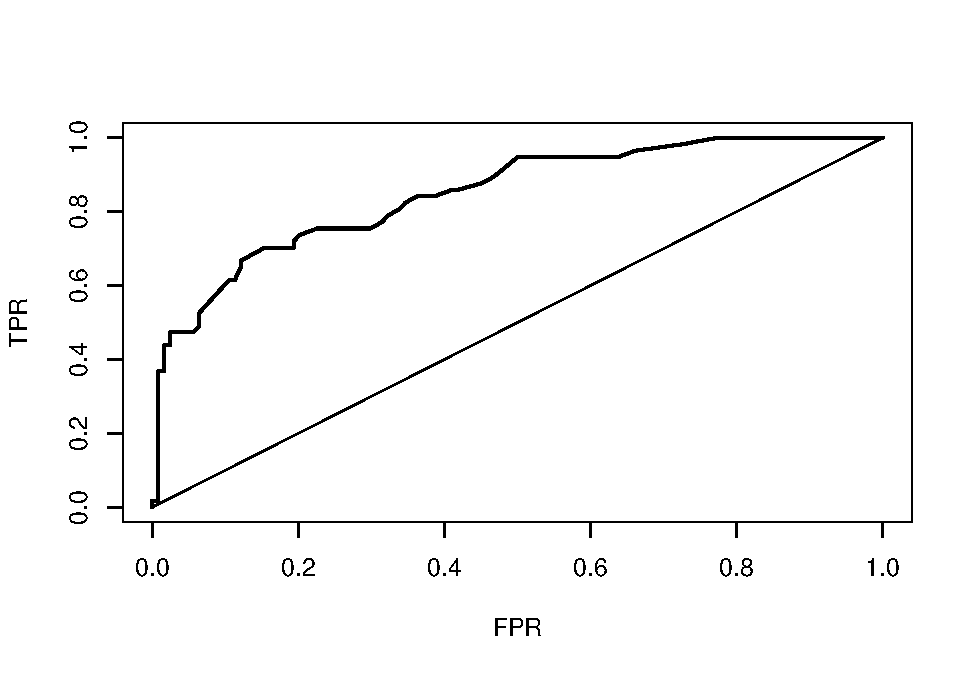
\includegraphics{Homework_2_files/figure-latex/unnamed-chunk-18-1.pdf}

AUC using manual calculation is 0.8488964.

Best Threshold value using method 1 is \{Threshold = 0.320000,fpr =
0.201613,tpr = 0.736842,auc = 0.767615, dist = 0.331511\}

Best Threshold value using method 2 is \{Threshold = 0.370000,fpr =
0.153226,tpr = 0.701754,auc = 0.774264, dist = 0.335304\}

\begin{itemize}
\item
  \begin{enumerate}
  \def\labelenumi{\arabic{enumi})}
  \setcounter{enumi}{1}
  \tightlist
  \item
    when cut-off interval is threshold(0,1,0.001) -\textgreater{} value
    is exact to what pROC predicts
  \end{enumerate}
\end{itemize}

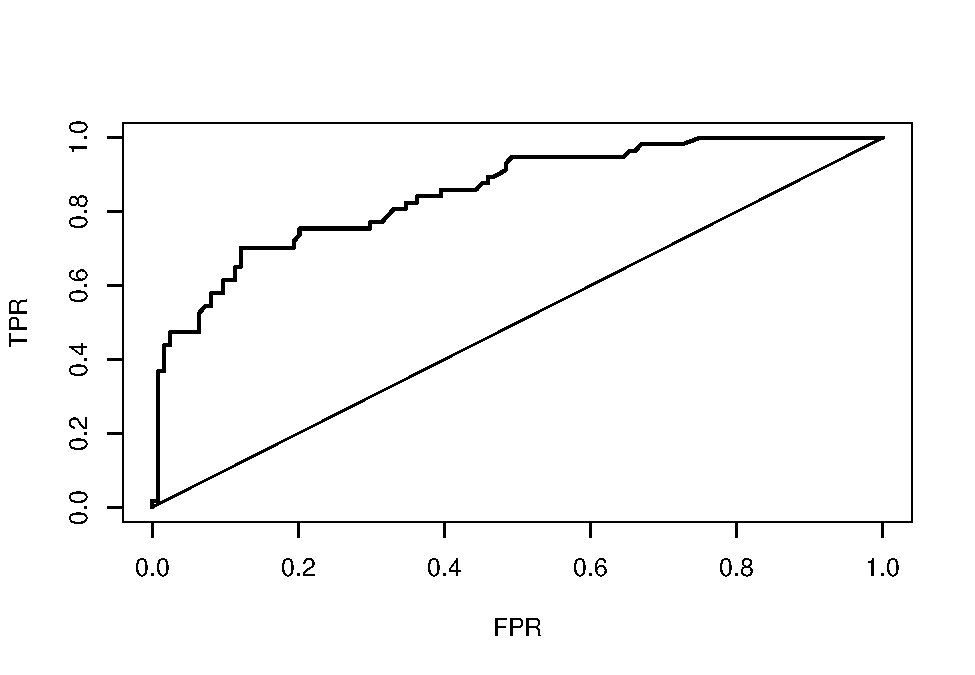
\includegraphics{Homework_2_files/figure-latex/unnamed-chunk-19-1.pdf}

AUC using manual calculation is 0.850382.

Best Threshold value using method 1 is \{Threshold = 0.316000,fpr =
0.201613,tpr = 0.754386,auc = 0.776387, dist = 0.317764\}

Best Threshold value using method 2 is \{Threshold = 0.374000,fpr =
0.120968,tpr = 0.701754,auc = 0.790393, dist = 0.321844\}

\clearpage

\section{\texorpdfstring{Investigation of \texttt{caret}
package}{Investigation of caret package}}\label{investigation-of-caret-package}

\subsection{confusionMatrix function}\label{confusionmatrix-function}

The results of the caret confusionMatrix function is below.

Here, the accuracy is rounded up to 4 decimal places. The confusion
matrix has rows that represent the predicted classes and columns that
represent the actual classes.

\begin{table}[ht]
\centering
\begin{tabular}{rrr}
  \hline
 & 0 & 1 \\ 
  \hline
0 & 119 &   5 \\ 
  1 &  30 &  27 \\ 
   \hline
\end{tabular}
\end{table}

\subsection{Sensitivity and Specificity
functions}\label{sensitivity-and-specificity-functions}

Sensitivity and specificity functions in the caret package take in only
two inputs - predicted and actual. On the other hand, the sensitivity
and specificity functions we created take in 5 outputs - the entire data
frame, preidicted variables, actual variables, the positive values, and
negative values.

The results of the Sensitivity function is below:

{[}1{]} ``Sensitivity provided by caret pacakge is 0.798657718120805''

The results of the Specificity function is below:

{[}1{]} ``Specificity provided by caret pacakge is 0.84375''

\pagebreak

\section{\texorpdfstring{Investigation of the \texttt{pROC} R
package.}{Investigation of the pROC R package.}}\label{investigation-of-the-proc-r-package.}

We used the \texttt{pROC} R package to generate an ROC curve for the
data set.

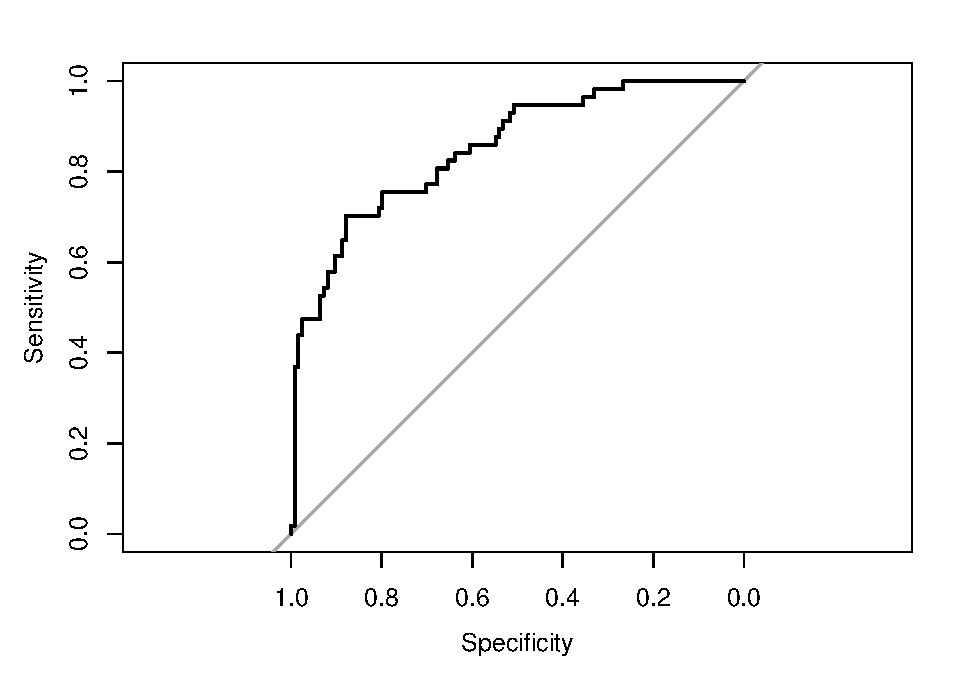
\includegraphics{Homework_2_files/figure-latex/unnamed-chunk-23-1.pdf}

\begin{verbatim}
## 
## Call:
## roc.default(response = dfData$class, predictor = dfData$scored.probability)
## 
## Data: dfData$scored.probability in 124 controls (dfData$class 0) < 57 cases (dfData$class 1).
## Area under the curve: 0.8503
\end{verbatim}

Best Threshold value using pROC package is \{Threshold = 0.375117,fpr =
0.120968,tpr = 0.701754\}

Note: The second method (using auc) predicts better than first method
(using distance from (0,1))

\newpage

\section{Appendix A}\label{appendix-a}

\subsection{Session Info}\label{session-info}

\begin{itemize}\raggedright
  \item R version 3.3.1 (2016-06-21), \verb|x86_64-w64-mingw32|
  \item Locale: \verb|LC_COLLATE=English_United States.1252|, \verb|LC_CTYPE=English_United States.1252|, \verb|LC_MONETARY=English_United States.1252|, \verb|LC_NUMERIC=C|, \verb|LC_TIME=English_United States.1252|
  \item Base packages: base, datasets, graphics, grDevices,
    methods, stats, utils
  \item Other packages: caret~6.0-71, dplyr~0.5.0, formatR~1.4,
    ggplot2~2.1.0, knitr~1.14, lattice~0.20-34, pacman~0.4.1,
    pander~0.6.0, pROC~1.8, purrr~0.2.2, readr~1.0.0,
    scales~0.4.0, tibble~1.2, tidyr~0.6.0, tidyverse~1.0.0,
    xtable~1.8-2
  \item Loaded via a namespace (and not attached): assertthat~0.1,
    car~2.1-3, class~7.3-14, codetools~0.2-15, colorspace~1.2-6,
    DBI~0.5-1, digest~0.6.10, e1071~1.6-7, evaluate~0.9,
    foreach~1.4.3, grid~3.3.1, gtable~0.2.0, htmltools~0.3.5,
    iterators~1.0.8, lme4~1.1-12, magrittr~1.5, MASS~7.3-45,
    Matrix~1.2-7.1, MatrixModels~0.4-1, mgcv~1.8-15, minqa~1.2.4,
    munsell~0.4.3, nlme~3.1-128, nloptr~1.0.4, nnet~7.3-12,
    parallel~3.3.1, pbkrtest~0.4-6, plyr~1.8.4, quantreg~5.29,
    R6~2.2.0, Rcpp~0.12.7, reshape2~1.4.1, rmarkdown~1.0,
    SparseM~1.72, splines~3.3.1, stats4~3.3.1, stringi~1.1.2,
    stringr~1.1.0, tools~3.3.1, yaml~2.1.13
\end{itemize}

\subsection{Data Table}\label{data-table}

\begin{longtable}[c]{@{}ccc@{}}
\toprule
class & scored.class & scored.probability\tabularnewline
\midrule
\endhead
0 & 0 & 0.3284523\tabularnewline
0 & 0 & 0.2731904\tabularnewline
1 & 0 & 0.1096604\tabularnewline
0 & 0 & 0.0559984\tabularnewline
0 & 0 & 0.1004907\tabularnewline
0 & 0 & 0.0551546\tabularnewline
0 & 0 & 0.1071154\tabularnewline
0 & 0 & 0.4599474\tabularnewline
0 & 0 & 0.1170237\tabularnewline
0 & 0 & 0.3153632\tabularnewline
0 & 0 & 0.1251892\tabularnewline
0 & 0 & 0.2706248\tabularnewline
0 & 0 & 0.2098096\tabularnewline
0 & 0 & 0.0935859\tabularnewline
1 & 1 & 0.8848457\tabularnewline
1 & 0 & 0.3966522\tabularnewline
0 & 1 & 0.8913949\tabularnewline
1 & 1 & 0.5345490\tabularnewline
1 & 1 & 0.9463342\tabularnewline
0 & 0 & 0.1449162\tabularnewline
0 & 0 & 0.2176380\tabularnewline
0 & 0 & 0.0752136\tabularnewline
0 & 0 & 0.0884325\tabularnewline
0 & 0 & 0.3034682\tabularnewline
1 & 1 & 0.7244800\tabularnewline
1 & 0 & 0.2749737\tabularnewline
1 & 0 & 0.4248648\tabularnewline
1 & 0 & 0.4309255\tabularnewline
0 & 0 & 0.0232280\tabularnewline
0 & 0 & 0.0459608\tabularnewline
0 & 0 & 0.1279853\tabularnewline
0 & 0 & 0.2993371\tabularnewline
1 & 0 & 0.4590950\tabularnewline
0 & 0 & 0.1047958\tabularnewline
1 & 1 & 0.8630918\tabularnewline
1 & 1 & 0.6399750\tabularnewline
0 & 0 & 0.3581843\tabularnewline
0 & 0 & 0.3721647\tabularnewline
1 & 1 & 0.8111032\tabularnewline
0 & 0 & 0.1681274\tabularnewline
0 & 0 & 0.1512780\tabularnewline
0 & 0 & 0.1070070\tabularnewline
0 & 0 & 0.1879614\tabularnewline
0 & 0 & 0.1371971\tabularnewline
0 & 0 & 0.3004749\tabularnewline
0 & 0 & 0.1368871\tabularnewline
0 & 0 & 0.0978691\tabularnewline
0 & 0 & 0.0629070\tabularnewline
1 & 0 & 0.2694193\tabularnewline
0 & 0 & 0.4885428\tabularnewline
0 & 0 & 0.3717580\tabularnewline
1 & 0 & 0.0994799\tabularnewline
0 & 0 & 0.0865623\tabularnewline
0 & 0 & 0.1752894\tabularnewline
1 & 0 & 0.4693790\tabularnewline
1 & 1 & 0.6165544\tabularnewline
0 & 0 & 0.0998279\tabularnewline
1 & 1 & 0.6891771\tabularnewline
0 & 0 & 0.2552862\tabularnewline
1 & 1 & 0.8505433\tabularnewline
1 & 0 & 0.1688625\tabularnewline
0 & 0 & 0.0972415\tabularnewline
0 & 0 & 0.2483691\tabularnewline
0 & 0 & 0.1815610\tabularnewline
0 & 0 & 0.2399936\tabularnewline
0 & 0 & 0.4045589\tabularnewline
0 & 0 & 0.3583026\tabularnewline
0 & 0 & 0.1506308\tabularnewline
1 & 0 & 0.4865383\tabularnewline
1 & 1 & 0.6150348\tabularnewline
0 & 0 & 0.3544895\tabularnewline
1 & 0 & 0.1731396\tabularnewline
1 & 0 & 0.2596111\tabularnewline
1 & 1 & 0.6989399\tabularnewline
0 & 0 & 0.2986016\tabularnewline
0 & 0 & 0.1042313\tabularnewline
0 & 0 & 0.2110528\tabularnewline
0 & 0 & 0.0654278\tabularnewline
0 & 0 & 0.0505143\tabularnewline
0 & 0 & 0.1086797\tabularnewline
0 & 0 & 0.0786895\tabularnewline
1 & 1 & 0.6812876\tabularnewline
1 & 0 & 0.3771203\tabularnewline
0 & 0 & 0.1627077\tabularnewline
0 & 0 & 0.3521508\tabularnewline
1 & 0 & 0.4754964\tabularnewline
0 & 0 & 0.1356581\tabularnewline
0 & 0 & 0.1339198\tabularnewline
0 & 1 & 0.5224711\tabularnewline
0 & 0 & 0.2593819\tabularnewline
0 & 0 & 0.0994674\tabularnewline
0 & 0 & 0.1271923\tabularnewline
1 & 0 & 0.3764462\tabularnewline
0 & 1 & 0.5208823\tabularnewline
1 & 1 & 0.7605921\tabularnewline
1 & 0 & 0.2089265\tabularnewline
1 & 0 & 0.2333521\tabularnewline
0 & 0 & 0.2059407\tabularnewline
0 & 0 & 0.1156596\tabularnewline
0 & 0 & 0.0839931\tabularnewline
1 & 0 & 0.1177312\tabularnewline
1 & 1 & 0.7170364\tabularnewline
0 & 0 & 0.1292900\tabularnewline
0 & 0 & 0.4368037\tabularnewline
0 & 0 & 0.2815537\tabularnewline
1 & 1 & 0.5919838\tabularnewline
1 & 1 & 0.8472932\tabularnewline
0 & 0 & 0.3151556\tabularnewline
0 & 0 & 0.1373101\tabularnewline
0 & 0 & 0.1680963\tabularnewline
0 & 0 & 0.0506711\tabularnewline
0 & 0 & 0.4983591\tabularnewline
1 & 0 & 0.4548143\tabularnewline
0 & 0 & 0.4504421\tabularnewline
1 & 0 & 0.1814974\tabularnewline
0 & 0 & 0.2942037\tabularnewline
1 & 0 & 0.4094483\tabularnewline
1 & 0 & 0.3167683\tabularnewline
0 & 0 & 0.1969549\tabularnewline
0 & 0 & 0.0627996\tabularnewline
1 & 1 & 0.8833591\tabularnewline
0 & 0 & 0.0993645\tabularnewline
1 & 0 & 0.4088370\tabularnewline
0 & 0 & 0.3624922\tabularnewline
0 & 0 & 0.0799184\tabularnewline
1 & 1 & 0.6172762\tabularnewline
0 & 0 & 0.2235817\tabularnewline
0 & 0 & 0.3013863\tabularnewline
0 & 0 & 0.0661091\tabularnewline
1 & 0 & 0.1670290\tabularnewline
0 & 0 & 0.2970645\tabularnewline
0 & 1 & 0.6276502\tabularnewline
0 & 0 & 0.2036287\tabularnewline
0 & 0 & 0.4574735\tabularnewline
0 & 0 & 0.3722721\tabularnewline
1 & 1 & 0.6357807\tabularnewline
0 & 0 & 0.0837734\tabularnewline
0 & 0 & 0.1519378\tabularnewline
0 & 0 & 0.0532099\tabularnewline
1 & 1 & 0.5486644\tabularnewline
0 & 0 & 0.4946261\tabularnewline
0 & 0 & 0.2353255\tabularnewline
0 & 0 & 0.1831519\tabularnewline
0 & 0 & 0.0641505\tabularnewline
0 & 0 & 0.0859556\tabularnewline
0 & 0 & 0.3737878\tabularnewline
0 & 0 & 0.4128094\tabularnewline
1 & 1 & 0.8304976\tabularnewline
0 & 0 & 0.1314538\tabularnewline
0 & 0 & 0.0661406\tabularnewline
0 & 0 & 0.1009617\tabularnewline
0 & 0 & 0.0286396\tabularnewline
0 & 0 & 0.2696404\tabularnewline
1 & 0 & 0.3281420\tabularnewline
0 & 0 & 0.1493509\tabularnewline
1 & 0 & 0.4555714\tabularnewline
0 & 0 & 0.0809498\tabularnewline
0 & 0 & 0.0347143\tabularnewline
1 & 1 & 0.6614750\tabularnewline
0 & 0 & 0.0659893\tabularnewline
0 & 0 & 0.1397903\tabularnewline
0 & 0 & 0.0474267\tabularnewline
0 & 0 & 0.0266070\tabularnewline
1 & 1 & 0.7825946\tabularnewline
0 & 0 & 0.1418285\tabularnewline
0 & 0 & 0.2850303\tabularnewline
1 & 0 & 0.3388554\tabularnewline
1 & 0 & 0.1626446\tabularnewline
0 & 1 & 0.5649062\tabularnewline
0 & 0 & 0.0562242\tabularnewline
0 & 0 & 0.1891168\tabularnewline
0 & 0 & 0.1707249\tabularnewline
0 & 0 & 0.1608049\tabularnewline
1 & 0 & 0.2457727\tabularnewline
0 & 0 & 0.1099905\tabularnewline
1 & 1 & 0.6764516\tabularnewline
0 & 0 & 0.3114196\tabularnewline
1 & 1 & 0.7072096\tabularnewline
1 & 1 & 0.8882766\tabularnewline
0 & 0 & 0.4224679\tabularnewline
0 & 0 & 0.1199810\tabularnewline
\bottomrule
\end{longtable}

\subsection{R source code}\label{r-source-code}

Please see
\href{https://github.com/ChristopheHunt/DATA-621-Group-1/blob/master/Homework\%202/Homework\%202.Rmd}{Homework
2.rmd} on GitHub for source code.

\url{https://github.com/ChristopheHunt/DATA-621-Group-1/blob/master/Homework\%202/Homework\%202.Rmd}.

\end{document}
